\documentclass{article}
\usepackage{graphicx}
\usepackage{hyperref}
\usepackage{tabularx}
\usepackage{tcolorbox}
\usepackage[table]{xcolor}
\usepackage{booktabs} 
\usepackage{enumitem} 
\usepackage{float}    



%\title{\textbf{Breaking Bread}}
%\author{Tommaso Ticci, Guillermo Caceres}
%\date{Aprile 2025}
%\renewcommand{\contentsname}{Indice}


\begin{document}

\begin{titlepage}
    \centering
    \includegraphics[width=0.4\textwidth]{imgs/Logo_unifi.jpg}\par\vspace{1cm}
    {\Large \textsc{Università degli Studi di Firenze}}\\
    {\large Dipartimento di Ingegneria dell'Informazione}\par\vspace{1cm}
    \rule{\linewidth}{0.5mm} \\[0.4cm]
    {\huge \textbf{Breaking Bread}}\\[0.2cm]
    {\Large Software per la gestione di ordini di un Fast-Food}\\
    \rule{\linewidth}{0.5mm} \\[1.5cm]

    \begin{flushleft}
        \textbf{Autori:}\\
        Tommaso Ticci \hspace{2cm} Guillermo Caceres\\
        \textbf{N. Matricola:} \\
        7110440\hspace{3.3cm}7111172\\[1cm]
        
        \textbf{Corso:} Ingegneria del Software\\[0.5cm]
        \textbf{Docente:} Enrico Vicario\\[0.5cm]
        \textbf{Anno Accademico:} 2024/2025
    \end{flushleft}
\end{titlepage}



\clearpage 

% Indice automatico(non toccare!!!)
\tableofcontents
\newpage

% ===== Sezioni  =====
\section{Introduzione}
Progetto realizzato per il superamento del corso di Ingegneria del Software e Laboratorio di Informatica del Corso di Laurea in Ingegneria Informatica. Il progetto consiste in un sistema di classi Java per la gestione dei menu e degli ordini di un fast-food. Realizzato da Tommaso Ticci mat. 7110440 e Guillermo Caceres mat. 7111172. Il progetto è disponibile sulla repository GitHub all'indirizzo:\\ https://github.com/TommasoTicci/BreakingBread.git

\subsection{Descrizione del progetto}
Il progetto permette agli utenti di effettuare ordini dal menu di un fast-food e di gestire i propri ordini. L'utente amministratore può organizzare il menu, inserendo o rimuovendo pietanze, e gestire gli ordini, gli utenti e i loro metodi di pagamento attraverso un'interfaccia dedicata. L'admin ha inoltre accesso a metodi di gestione diretta del database.


\subsection{Struttura del progetto e tecnologie usate}
Il progetto è interamente realizzato in Java. La gestione dei dati è affidata al DBMS PostgreSQL, integrato mediante l'utilizzo del pattern DAO, che permette di separare la logica di business dalla logica di persistenza dei dati. A questo scopo, il progetto è stato strutturato nei package: \textbf{Business Logic}, \textbf{Domain Model} e \textbf{ORM}.\\ La progettazione è stata realizzata attraverso diagrammi Use Case Diagram e Class Diagram secondo lo standard UML. Per la fase di testing è stato utilizzato JUnit. \\
Programmi utilizzati:
\begin{itemize}
    \item {\textbf{IntelliJ IDEA}}: IDE per la scrittura e compilazione del codice Java
    \item {\textbf{GitHub}}: piattaforma online per il versionamento e condivisione del codice
    \item {\textbf{StarUML}}: software per la creazione di vari diagrammi
    \item {\textbf{Draw.io}}: web app per la creazione di vari diagrammi
    \item {\textbf{Lunacy}}: software per la creazione di mock-ups
\end{itemize}
\\

\begin{figure}[H]
    \centering
    \includegraphics[width=0.9\linewidth]{imgs/PackageDependecy.png}
    \caption{Package Dependency}
    \label{PackageDependecy}
\end{figure}

\subsection{Utilizzo di Strumenti AI}
Durante la scrittura del codice sono state usate tecnologie generative AI come \textbf{GitHub Copilot}, utilizzate principalmente per la scrittura veloce di codice semplice e per la realizzazione di classi poco complesse. \\


\section{Progettazione}

\subsection{Use Case Diagram}
La progettazione è stata realizzata con uno Use Case Diagram (figura \ref{useCaseDiagram}), dal quale si notano i ruoli dello "User" e del "Admin" e le operazioni che questi posso fare. I numeri presenti in alcuni nodi del grafico rappresentano il numero del template collegato a tale operazione.

\begin{figure}[h]
    \hspace*{-2.5cm}
    \includegraphics[width=1.45\textwidth]{imgs/UseCaseDiagramVer2.png}
    \caption{Use Case Diagram}
    \label{useCaseDiagram}
\end{figure}

\clearpage

\subsection{Use Case Template} \label{subsec:use-case-template}
%to be modified
    Di seguito sono riportati i template di alcuni dei casi d'uso, in ciascuno possiamo trovare: una breve descrizione,
    il livello del caso d'uso, gli attori coinvolti, le pre-condizioni, le post-condizioni, il flusso base e i flussi alternativi. \\

\begin{figure}[!h]
    \centering
    \includegraphics[width=0.75\linewidth]{imgs/Test.png}
    \caption{Test}
    \centering
    \label{Test}
\end{figure}

\newpage


% Use Case Template 1
            \begin{table}%[h]
                \centering
                \small
                \begin{tabularx}{\textwidth}{|lX|}
                    %\bottomrule
                    \multicolumn{1}{l}{\rowcolor{grey!20} \textbf{Use Case \#1}} & \multicolumn{1}{l}{\textbf{Log In}} \\
                    \bottomrule
                    \rowcolor{white} \textbf{Brief Description} & L'utente accede al sistema (MK\#01) \\
                    %\midrule
                    \rowcolor{blue!10} \textbf{Level} & User goal \\
                    %\midrule
                    \rowcolor{white} \textbf{Actors} & User, Admin \\
                    %\midrule
                    \rowcolor{blue!10} \textbf{Pre-conditions} & L'utente deve essere nella pagina di login del programma \\
                    %\midrule
                    \rowcolor{white} \textbf{Basic Flow} & \begin{description}[nosep,before=\leavevmode\vspace*{-1\baselineskip},after=\leavevmode\vspace*{-1\baselineskip}]
                                                                \item [1.] L'utente inserisce le proprie credenziali di
                                                                accesso
                                                                \item [2.] L'utente preme il pulsante di conferma per accedere al sistema
                                                                \item [3.] Il sistema controlla che le credenziali siano corrette e che ci sia corrispondenza sul database
                                                                \item [4.] Il sistema autentica l'utente (TST\#01)
                                                            \end{description} \\
                     %\midrule
                    \rowcolor{blue!10} \textbf{Alternative Flows} & \begin{description}[nosep,before=\leavevmode\vspace*{-1\baselineskip},after=\leavevmode\vspace*{-1\baselineskip}]
                                                                        \item [3a.] Se le credenziali fornite sono errate, il sistema mostra un messaggio di errore all'utente
                                                                        \item [4a.] Se a fare l'accesso è l'admin, il sistema lo reindirizza alla Admin Page (MK\#06)
                                                                    \end{description} \\
                    %\midrule
                    \rowcolor{white} \textbf{Post-conditions} & L'utente ha accesso al sistema \\
                    %\bottomrule
                    \toprule
                \end{tabularx}
                %}
                %\captionsetup{font=small,labelfont=bf}
                \caption{Use Case Template 1 (Log In)}
                \label{tab:use-case-template-1}
            \end{table}

% Use Case Template 2
            \begin{table}%[h]
                \centering
                \small
                \begin{tabularx}{\textwidth}{|lX|}
                    %\bottomrule
                    \multicolumn{1}{l}{\rowcolor{grey!20} \textbf{Use Case \#2}} & \multicolumn{1}{l}{\textbf{Register}} \\
                    \bottomrule
                    \rowcolor{white} \textbf{Brief Description} & L'utente crea un nuovo account e si registra al sistema (MK\#02) \\
                    %\midrule
                    \rowcolor{blue!10} \textbf{Level} & User goal \\
                    %\midrule
                    \rowcolor{white} \textbf{Actors} & User \\
                    %\midrule
                    \rowcolor{blue!10} \textbf{Pre-conditions} & L'utente deve essere nella pagina di registrazione \\
                    %\midrule
                    \rowcolor{white} \textbf{Basic Flow} & \begin{description}[nosep,before=\leavevmode\vspace*{-1\baselineskip},after=\leavevmode\vspace*{-1\baselineskip}]
                                                                \item [1.] L'utente inserisce i propri dati e le sue nuove credenziali
                                                                \item [2.] L'utente preme il pulsante di conferma per registrarsi al sistema
                                                                \item [3.] Il sistema controlla che i dati forniti siano corretti
                                                                \item [4.] Il sistema registra il nuovo utente nel database
                                                                (TST\#02)
                                                            \end{description} \\
                     %\midrule
                    \rowcolor{blue!10} \textbf{Alternative Flows} & \begin{description}[nosep,before=\leavevmode\vspace*{-1\baselineskip},after=\leavevmode\vspace*{-1\baselineskip}]
                                                                        \item [1a.] L'utente può inserire il metodo di pagamento, non richiesto obbligatoriamente al momento della registrazione
                                                                        \item [3a.] Se l'utente inserisce dati errati o se l'username o l'email sono già utilizzati da un altro utente, il sistema mostra un messaggio di errore
                                                                    \end{description} \\
                    %\midrule
                    \rowcolor{white} \textbf{Post-conditions} & L'utente è registrato nel sistema \\
                    %\bottomrule
                    \toprule
                \end{tabularx}
                %}
                %\captionsetup{font=small,labelfont=bf}
                \caption{Use Case Template 2 (Register)}
                \label{tab:use-case-template-2}
            \end{table}

% Use Case Template 3
            \begin{table}%[h]
                \centering
                \small
                \begin{tabularx}{\textwidth}{|lX|}
                    %\bottomrule
                    \multicolumn{1}{l}{\rowcolor{grey!20} \textbf{Use Case \#3}} & \multicolumn{1}{l}{\textbf{Add Items to Cart}} \\
                    \bottomrule
                    \rowcolor{white} \textbf{Brief Description} & L'utente inserisce una pietanza nel suo carrello \\
                    %\midrule
                    \rowcolor{blue!10} \textbf{Level} & User goal \\
                    %\midrule
                    \rowcolor{white} \textbf{Actors} & User \\
                    %\midrule
                    \rowcolor{blue!10} \textbf{Pre-conditions} & L'utente deve essere nella pagina del proprio carrello (MK\#04) \\
                    %\midrule
                    \rowcolor{white} \textbf{Basic Flow} & \begin{description}[nosep,before=\leavevmode\vspace*{-1\baselineskip},after=\leavevmode\vspace*{-1\baselineskip}]
                                                                \item [1.] L'utente preme il pulsante "Add Item"
                                                                \item [2.] L'utente digita l'id della pietanza che vuole aggiungere al carrello
                                                                \item [3.] L'utente digita la quantità di tale pietanza
                                                                \item [4.] Il sistema controlla i dati inseriti (TST\#03)
                                                            \end{description} \\
                     %\midrule
                    \rowcolor{blue!10} \textbf{Alternative Flows} & \begin{description}[nosep,before=\leavevmode\vspace*{-1\baselineskip},after=\leavevmode\vspace*{-1\baselineskip}]
                                                                        \item [4a.] Se l'utente inserisce un id non esistente o una quantità negativa, il sistema mostra un messaggio di errore 
                                                                        \item [4b.] Se l'utente inserisce una quantità pari a zero, il sistema non inserisce nessuna pietanza
                                                                    \end{description} \\
                    %\midrule
                    \rowcolor{white} \textbf{Post-conditions} & La pietanza viene aggiunta al carrello \\
                    %\bottomrule
                    \toprule
                \end{tabularx}
                %}
                %\captionsetup{font=small,labelfont=bf}
                \caption{Use Case Template 3 (Add Items to Cart)}
                \label{tab:use-case-template-3}
            \end{table}

% Use Case Template 4
            \begin{table}%[h]
                \centering
                \small
                \begin{tabularx}{\textwidth}{|lX|}
                    %\bottomrule
                    \multicolumn{1}{l}{\rowcolor{grey!20} \textbf{Use Case \#4}} & \multicolumn{1}{l}{\textbf{Pay Order}} \\
                    \bottomrule
                    \rowcolor{white} \textbf{Brief Description} & L'utente effettua il pagamento dell'ordine nel carrello (MK\#05) \\
                    %\midrule
                    \rowcolor{blue!10} \textbf{Level} & Function \\
                    %\midrule
                    \rowcolor{white} \textbf{Actors} & User \\
                    %\midrule
                    \rowcolor{blue!10} \textbf{Pre-conditions} & L'utente ha premuto il pulsante di conferma ordine nella pagina del carrello (MK\#04) \\
                    %\midrule
                    \rowcolor{white} \textbf{Basic Flow} & \begin{description}[nosep,before=\leavevmode\vspace*{-1\baselineskip},after=\leavevmode\vspace*{-1\baselineskip}]
                                                                \item [1.] Il sistema mostra il riepilogo dell'ordine
                                                                \item [2.] L'utente digita il CVV della carta collegata
                                                                \item [3.] Il sistema verifica i dati ed esegue il pagamento
                                                                \item [4.] Il sistema conferma all'utente che il pagamento è stato effettuato con successo (TST\#04)
                                                            \end{description} \\
                     %\midrule
                    \rowcolor{blue!10} \textbf{Alternative Flows} & \begin{description}[nosep,before=\leavevmode\vspace*{-1\baselineskip},after=\leavevmode\vspace*{-1\baselineskip}]
                                                                        \item [1a.] Se il carrello è vuoto, il sistema mostra un messaggio di errore
                                                                        \item [1b.] Se l'utente non ha nessun metodo di pagamento associato all'account, il sistema mostra un messaggio di errore
                                                                        \item [3a.] Se l'utente inserisce dati errati, il sistema mostra un messaggio di errore
                                                                    \end{description} \\
                    %\midrule
                    \rowcolor{white} \textbf{Post-conditions} & L'ordine effettuato viene aggiunto nel sistema \\
                    %\bottomrule
                    \toprule
                \end{tabularx}
                %}
                %\captionsetup{font=small,labelfont=bf}
                \caption{Use Case Template 4 (Pay Order)}
                \label{tab:use-case-template-4}
            \end{table}

% Use Case Template 5
            \begin{table}%[h]
                \centering
                \small
                \begin{tabularx}{\textwidth}{|lX|}
                    %\bottomrule
                    \multicolumn{1}{l}{\rowcolor{grey!20} \textbf{Use Case \#5}} & \multicolumn{1}{l}{\textbf{Cancel Order}} \\
                    \bottomrule
                    \rowcolor{white} \textbf{Brief Description} & L'utente cancella un ordine dal sistema e riceve un rimborso \\
                    %\midrule
                    \rowcolor{blue!10} \textbf{Level} & User goal \\
                    %\midrule
                    \rowcolor{white} \textbf{Actors} & User \\
                    %\midrule
                    \rowcolor{blue!10} \textbf{Pre-conditions} & L'utente deve aver effettuato tale ordine \\
                    %\midrule
                    \rowcolor{white} \textbf{Basic Flow} & \begin{description}[nosep,before=\leavevmode\vspace*{-1\baselineskip},after=\leavevmode\vspace*{-1\baselineskip}]
                                                                \item [1.] L'utente digita l'id dell'ordine che vuole cancellare
                                                                \item [2.] Il sistema verifica l'id inserito
                                                                \item [3.] Il sistema effettua un rimborso all'utente
                                                                \item [4.] Il sistema cancella l'ordine e comunica all'utente il successo di tale operazione (TST\#05)
                                                            \end{description} \\
                     %\midrule
                    \rowcolor{blue!10} \textbf{Alternative Flows} & \begin{description}[nosep,before=\leavevmode\vspace*{-1\baselineskip},after=\leavevmode\vspace*{-1\baselineskip}]
                                                                        \item [2a.] Se l'id è inesistente oppure l'id dell'ordine esiste ma questo è stato effettuato da un altro utente, il sistema mostra un messaggio di errore
                                                                        \item [2b.] Se l'id dell'ordine ha corrispondenza, ma l'ordine ha uno status diverso da "Recieved", il sistema mostra un messaggio di errore
                                                                        \item [3a.] Se l'utente non ha nessun metodo di pagamento associato all'account, il sistema mostra un messaggio di errore
                                                                    \end{description} \\
                    %\midrule
                    \rowcolor{white} \textbf{Post-conditions} & L'ordine selezionato viene rimosso dal sistema e l'utente viene rimborsato \\
                    %\bottomrule
                    \toprule
                \end{tabularx}
                %}
                %\captionsetup{font=small,labelfont=bf}
                \caption{Use Case Template 5 (Cancel Order)}
                \label{tab:use-case-template-5}
            \end{table}

% Use Case Template 6
            \begin{table}%[h]
                \centering
                \small
                \begin{tabularx}{\textwidth}{|lX|}
                    %\bottomrule
                    \multicolumn{1}{l}{\rowcolor{grey!20} \textbf{Use Case \#6}} & \multicolumn{1}{l}{\textbf{Change Password}} \\
                    \bottomrule
                    \rowcolor{white} \textbf{Brief Description} & L'utente modifica la propria password \\
                    %\midrule
                    \rowcolor{blue!10} \textbf{Level} & User goal \\
                    %\midrule
                    \rowcolor{white} \textbf{Actors} & User \\
                    %\midrule
                    \rowcolor{blue!10} \textbf{Pre-conditions} & L'utente deve essere autenticato \\
                    %\midrule
                    \rowcolor{white} \textbf{Basic Flow} & \begin{description}[nosep,before=\leavevmode\vspace*{-1\baselineskip},after=\leavevmode\vspace*{-1\baselineskip}]
                                                                \item [1.] L'utente accede alle impostazioni del proprio account
                                                                \item [2.] L'utente seleziona l'opzione per la modifica della password
                                                                \item [3.] L'utente inserisce la nuova password
                                                                \item [4.] L'utente inserisce la conferma della nuova password
                                                                \item [5.] Il sistema controlla i dati inseriti
                                                                \item [6.] Il sistema aggiorna la password dell'utente  (TST\#06)
                                                            \end{description} \\
                     %\midrule
                    \rowcolor{blue!10} \textbf{Alternative Flows} & \begin{description}[nosep,before=\leavevmode\vspace*{-1\baselineskip},after=\leavevmode\vspace*{-1\baselineskip}]
                                                                        \item [5a.] Se la password è vuota o la conferma password non corrisponde alla nuova password, il sistema mostra un messaggio di errore
                                                                    \end{description} \\
                    %\midrule
                    \rowcolor{white} \textbf{Post-conditions} & La password dell'utente viene aggiornata \\
                    %\bottomrule
                    \toprule
                \end{tabularx}
                %}
                %\captionsetup{font=small,labelfont=bf}
                \caption{Use Case Template 6 (Change Password)}
                \label{tab:use-case-template-6}
            \end{table}

% Use Case Template 7
            \begin{table}%[h]
                \centering
                \small
                \begin{tabularx}{\textwidth}{|lX|}
                    %\bottomrule
                    \multicolumn{1}{l}{\rowcolor{grey!20} \textbf{Use Case \#7}} & \multicolumn{1}{l}{\textbf{Set Payment Method}} \\
                    \bottomrule
                    \rowcolor{white} \textbf{Brief Description} & L'utente inserisce un metodo di pagamento nel sistema  \\
                    %\midrule
                    \rowcolor{blue!10} \textbf{Level} & User goal \\
                    %\midrule
                    \rowcolor{white} \textbf{Actors} & User \\
                    %\midrule
                    \rowcolor{blue!10} \textbf{Pre-conditions} & L'utente deve essere autenticato \\
                    %\midrule
                    \rowcolor{white} \textbf{Basic Flow} & \begin{description}[nosep,before=\leavevmode\vspace*{-1\baselineskip},after=\leavevmode\vspace*{-1\baselineskip}]
                                                                \item [1.] L'utente accede alle impostazioni del proprio account
                                                                \item [2.] L'utente seleziona l'opzione per l'inserimento del metodo di pagamento
                                                                \item [3.] L'utente inserisce i dati del suo metodo di pagamento
                                                                \item [4.] Il sistema controlla i dati inseriti
                                                                \item [5.] Il sistema associa il nuovo metodo di pagamento all'account dell'utente (TST\#07)
                                                            \end{description} \\
                     %\midrule
                    \rowcolor{blue!10} \textbf{Alternative Flows} & \begin{description}[nosep,before=\leavevmode\vspace*{-1\baselineskip},after=\leavevmode\vspace*{-1\baselineskip}]
                                                                        \item [4a.] Se i dati inseriti sono invalidi, il sistema mostra un messaggio di errore
                                                                        \item [5a.] Se l'utente aveva già associato un metodo di pagamento, questo viene sostituito da quello nuovo
                                                                    \end{description} \\
                    %\midrule
                    \rowcolor{white} \textbf{Post-conditions} & Il nuovo metodo di pagamento viene associato all'account dell'utente \\
                    %\bottomrule
                    \toprule
                \end{tabularx}
                %}
                %\captionsetup{font=small,labelfont=bf}
                \caption{Use Case Template 7 (Set Payment Method)}
                \label{tab:use-case-template-7}
            \end{table}

% Use Case Template 8
            \begin{table}%[h]
                \centering
                \small
                \begin{tabularx}{\textwidth}{|lX|}
                    %\bottomrule
                    \multicolumn{1}{l}{\rowcolor{grey!20} \textbf{Use Case \#8}} & \multicolumn{1}{l}{\textbf{Add Item}} \\
                    \bottomrule
                    \rowcolor{white} \textbf{Brief Description} & L'admin aggiunge una nuova pietanza al menu (MK\#7) \\
                    %\midrule
                    \rowcolor{blue!10} \textbf{Level} & User goal \\
                    %\midrule
                    \rowcolor{white} \textbf{Actors} & Admin \\
                    %\midrule
                    \rowcolor{blue!10} \textbf{Pre-conditions} & L'admin deve essere autenticato dal sistema \\
                    %\midrule
                    \rowcolor{white} \textbf{Basic Flow} & \begin{description}[nosep,before=\leavevmode\vspace*{-1\baselineskip},after=\leavevmode\vspace*{-1\baselineskip}]
                                                                \item [1.] L'admin accede alle impostazioni del menu
                                                                \item [2.] L'admin seleziona l'opzione per l'aggiunta di una nuova pietanza
                                                                \item [3.] L'admin inserisce i dati e le informazioni della nuova pietanza (MK\#7)
                                                                \item [4.] Il sistema verifica i dati inseriti
                                                                \item [5.] Il sistema aggiunge la nuova pietanza al menu
                                                            \end{description} \\
                     %\midrule
                    \rowcolor{blue!10} \textbf{Alternative Flows} & \begin{description}[nosep,before=\leavevmode\vspace*{-1\baselineskip},after=\leavevmode\vspace*{-1\baselineskip}]
                                                                        \item [4a.] Se i dati inseriti sono invalidi, il sistema mostra un messaggio di errore
                                                                    \end{description} \\
                    %\midrule
                    \rowcolor{white} \textbf{Post-conditions} & La nuova pietanza viene aggiunta al menu \\
                    %\bottomrule
                    \toprule
                \end{tabularx}
                %}
                %\captionsetup{font=small,labelfont=bf}
                \caption{Use Case Template 8 (Add Item)}
                \label{tab:use-case-template-8}
            \end{table}

% Use Case Template 9
            \begin{table}%[h]
                \centering
                \small
                \begin{tabularx}{\textwidth}{|lX|}
                    %\bottomrule
                    \multicolumn{1}{l}{\rowcolor{grey!20} \textbf{Use Case \#9}} & \multicolumn{1}{l}{\textbf{Update Order Status}} \\
                    \bottomrule
                    \rowcolor{white} \textbf{Brief Description} & L'admin modifica lo stato di un ordine \\
                    %\midrule
                    \rowcolor{blue!10} \textbf{Level} & User goal \\
                    %\midrule
                    \rowcolor{white} \textbf{Actors} & Admin \\
                    %\midrule
                    \rowcolor{blue!10} \textbf{Pre-conditions} & L'admin deve essere autenticato dal sistema \\
                    %\midrule
                    \rowcolor{white} \textbf{Basic Flow} & \begin{description}[nosep,before=\leavevmode\vspace*{-1\baselineskip},after=\leavevmode\vspace*{-1\baselineskip}]
                                                                \item [1.] L'admin accede alla pagina di gestione degli ordini
                                                                \item [2.] L'admin seleziona l'opzione per la modifica dello stato di un ordine
                                                                \item [3.] L'admin inserisce l'id del'ordine che vuole modificare e il nuovo status
                                                                \item [4.] Il sistema verifica i dati inseriti
                                                                \item [5.] Il sistema modifica lo stato dell'ordine selezionato
                                                            \end{description} \\
                     %\midrule
                    \rowcolor{blue!10} \textbf{Alternative Flows} & \begin{description}[nosep,before=\leavevmode\vspace*{-1\baselineskip},after=\leavevmode\vspace*{-1\baselineskip}]
                                                                        \item [4a.] Se l'id o lo stato inseriti sono invalidi, il sistema mostra un messaggio di errore
                                                                    \end{description} \\
                    %\midrule
                    \rowcolor{white} \textbf{Post-conditions} & Lo stato dell'ordine selezionato viene modificato \\
                    %\bottomrule
                    \toprule
                \end{tabularx}
                %}
                %\captionsetup{font=small,labelfont=bf}
                \caption{Use Case Template 9 (Update Order Status)}
                \label{tab:use-case-template-9}
            \end{table}

% Use Case Template 10
            \begin{table}
                \centering
                \small
                \begin{tabularx}{\textwidth}{|lX|}
                    %\bottomrule
                    \multicolumn{1}{l}{\rowcolor{grey!20} \textbf{Use Case \#10}} & \multicolumn{1}{l}{\textbf{Reset Database}} \\
                    \bottomrule
                    \rowcolor{white} \textbf{Brief Description} & L'admin effettua il ripristino del database \\
                    %\midrule
                    \rowcolor{blue!10} \textbf{Level} & Function \\
                    %\midrule
                    \rowcolor{white} \textbf{Actors} & Admin \\
                    %\midrule
                    \rowcolor{blue!10} \textbf{Pre-conditions} & L'admin deve essere autenticato dal sistema \\
                    %\midrule
                    \rowcolor{white} \textbf{Basic Flow} & \begin{description}[nosep,before=\leavevmode\vspace*{-1\baselineskip},after=\leavevmode\vspace*{-1\baselineskip}]
                                                                \item [1.] L'admin accede alla pagina di gestione del database
                                                                \item [2.] L'admin seleziona l'opzione per il reset del database
                                                                \item [3.] L'admin reinserisce la password per confermare l'operazione
                                                                \item [4.] Il sistema esegue il ripristino del database
                                                            \end{description} \\
                     %\midrule
                    \rowcolor{blue!10} \textbf{Alternative Flows} & \begin{description}[nosep,before=\leavevmode\vspace*{-1\baselineskip},after=\leavevmode\vspace*{-1\baselineskip}]
                                                                        \item [3a.] Se la password inserita è errata, il sistema mostra un messaggio di errore
                                                                    \end{description} \\
                    %\midrule
                    \rowcolor{white} \textbf{Post-conditions} & Il database viene ripristinato con successo \\
                    %\bottomrule
                    \toprule
                \end{tabularx}
                %}
                %\captionsetup{font=small,labelfont=bf}
                \caption{Use Case Template 10 (Reset Database)}
                \label{tab:use-case-template-10}
            \end{table}
            \clearpage
            


            
            \renewcommand{\arraystretch}{1}

    \vspace{1cm}

\subsection{Navigation Diagram}
Il diagramma di navigazione (figura \ref{navigationDiagram}) descrive la struttura dell'applicazione, suddividendo le funzionalità tra utenti e amministratori. Dalla schermata iniziale, gli utenti possono accedere, registrarsi o entrare come admin. L'area utente permette di visualizzare il menu, gestire il carrello, controllare ordini e modificare il profilo. Gli amministratori hanno accesso a strumenti per gestire utenti, modificare il menu, monitorare ordini e intervenire sul database. Ogni sezione include sempre la possibilità di tornare indietro, garantendo un flusso intuitivo. Il sistema è progettato per coprire l'intero ciclo degli ordini, dall'acquisto alla gestione amministrativa. I numeri scritti sopra le
frecce corrispondono ai comandi da digitare tramite la CLI. Il numero \texttt{0} permette di ritornare alla pagina precedente o di chiudere il programma nel caso l'utente si trovi nella prima pagina (Breaking Bread).

\begin{figure}[H]
    \centering
    \hspace*{-2.5cm}
    \includegraphics[width=1.4\textwidth]{imgs/NavigationDiagram.png}%
    \caption{Navigation Diagram}
    \label{navigationDiagram}
\end{figure}

\newpage

\subsection{Mockups}
In seguito vengono mostrati alcuni Mockups dell'interfaccia del programma.

\setlength{\fboxsep}{0pt}
            \begin{figure}[H]
                \centering
                \resizebox{1\textwidth}{!}{
                \setlength{\fboxsep}{0pt}
                \tcbox[colframe=grey!20,colback=grey!20,boxsep=0mm,arc=1mm]{
                    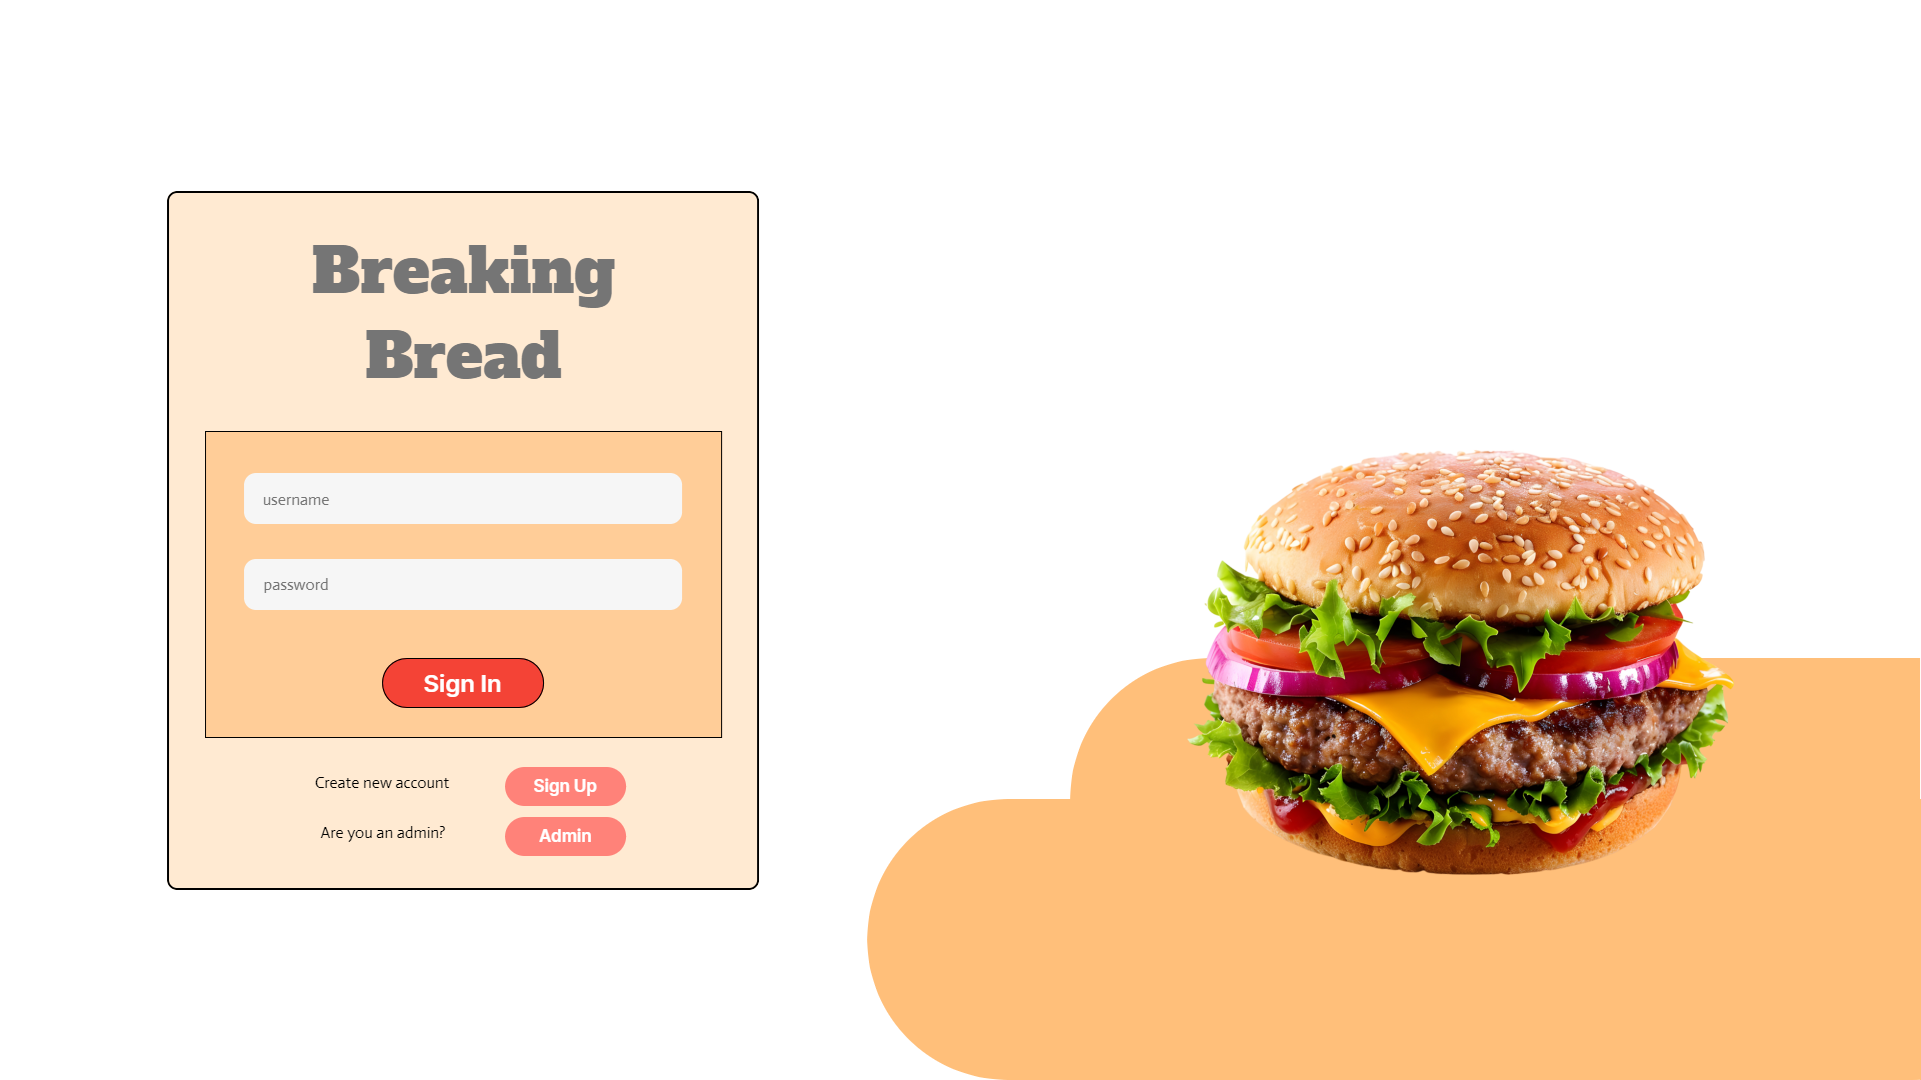
\includegraphics[width=\textwidth]{imgs/mockups/MK_1_LoginPage.png}
                }
                }
                \caption{Mockup della pagina iniziale di login - MK\#1}
                \label{fig:mk.1}
            \end{figure}
            
\setlength{\fboxsep}{0pt}
            \begin{figure}[H]
                \centering
                \resizebox{1\textwidth}{!}{
                \setlength{\fboxsep}{0pt}
                \tcbox[colframe=grey!20,colback=grey!20,boxsep=0mm,arc=1mm]{
                    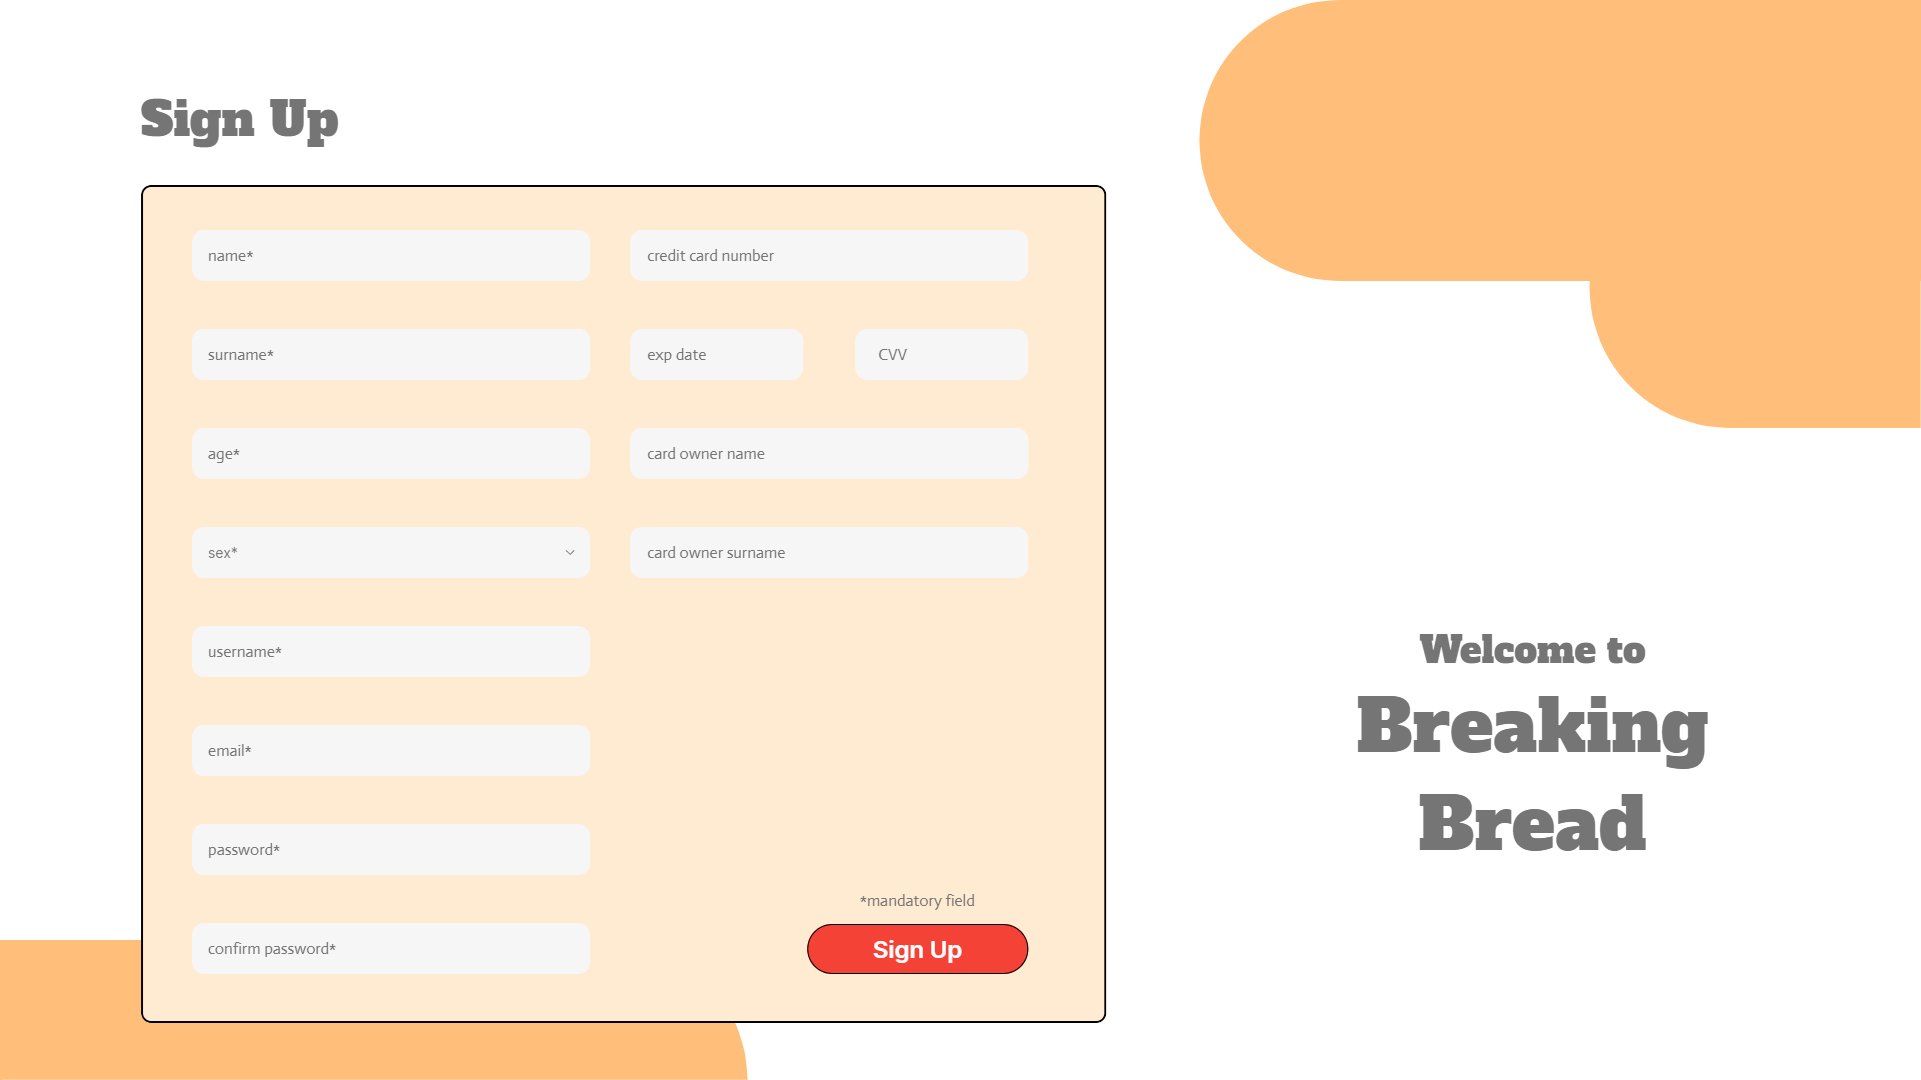
\includegraphics[width=\textwidth]{imgs/mockups/MK_2_RegisterPage.png}
                }
                }
                \caption{Mockup della pagina di registrazione - MK\#2}
                \label{fig:mk.2}
            \end{figure}

\setlength{\fboxsep}{0pt}
            \begin{figure}[H]
                \centering
                \resizebox{1\textwidth}{!}{
                \setlength{\fboxsep}{0pt}
                \tcbox[colframe=grey!20,colback=grey!20,boxsep=0mm,arc=1mm]{
                    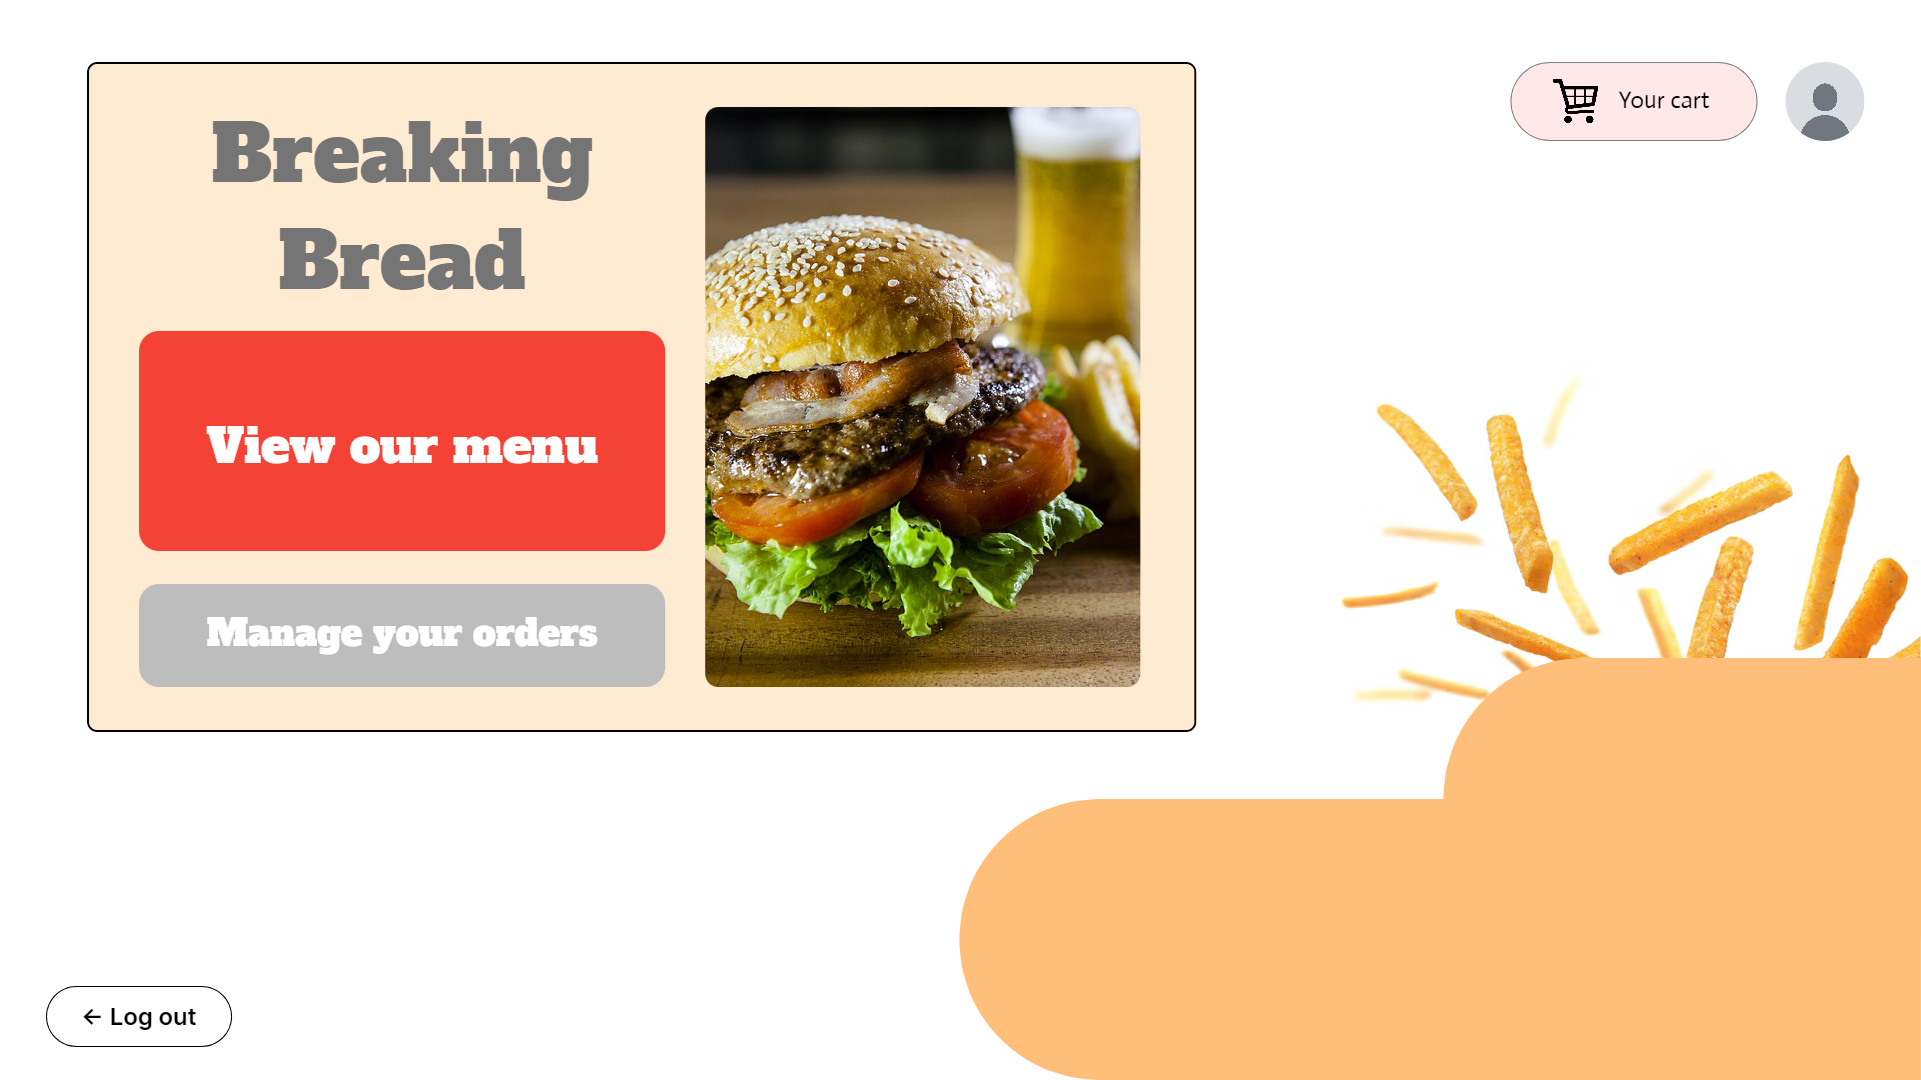
\includegraphics[width=\textwidth]{imgs/mockups/MK_3_UserPage.png}
                }
                }
                \caption{Mockup della homepage dell'utente  - MK\#3}
                \label{fig:mk.3}
            \end{figure}

\setlength{\fboxsep}{0pt}
            \begin{figure}[H]
                \centering
                \resizebox{1\textwidth}{!}{
                \setlength{\fboxsep}{0pt}
                \tcbox[colframe=grey!20,colback=grey!20,boxsep=0mm,arc=1mm]{
                    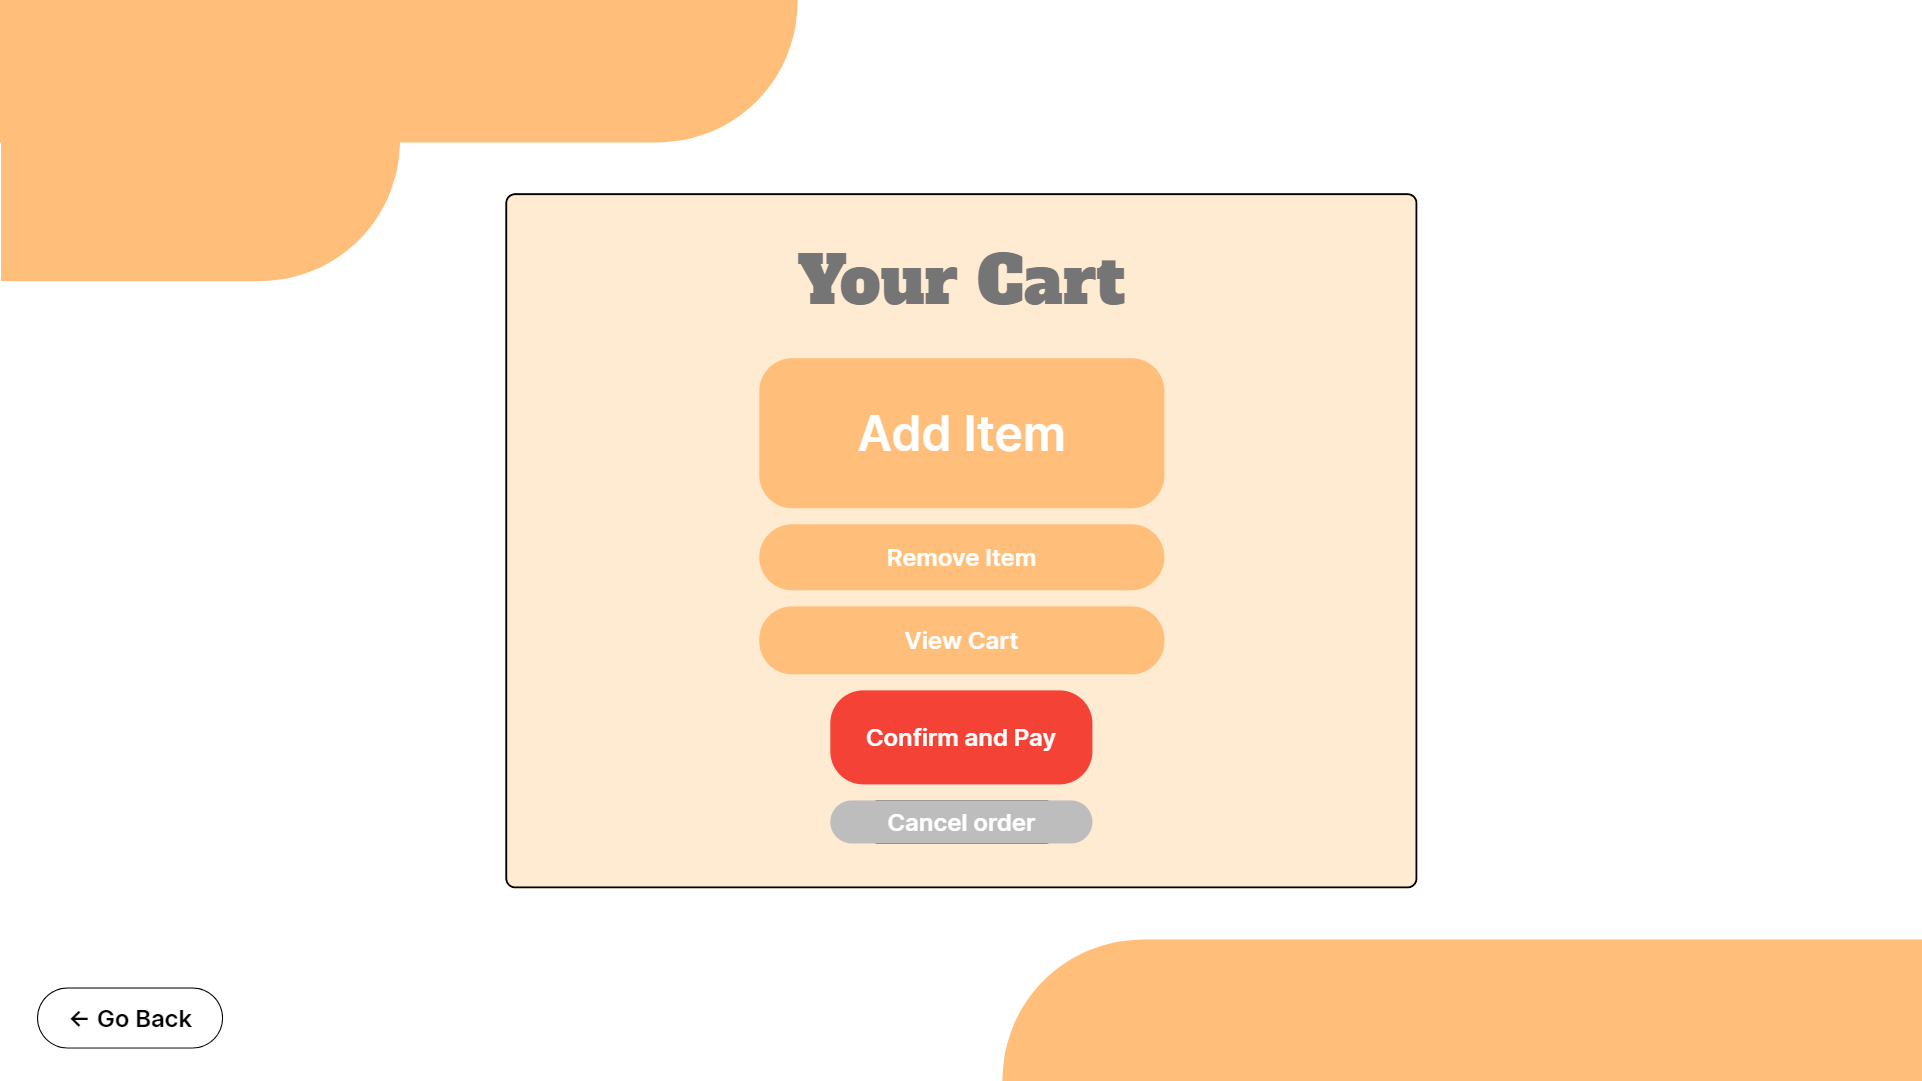
\includegraphics[width=\textwidth]{imgs/mockups/MK_4_CartPage.png}
                }
                }
                \caption{Mockup della pagina del carrello dell'utente - MK\#4}
                \label{fig:mk.4}
            \end{figure}

\setlength{\fboxsep}{0pt}
            \begin{figure}[H]
                \centering
                \resizebox{1\textwidth}{!}{
                \setlength{\fboxsep}{0pt}
                \tcbox[colframe=grey!20,colback=grey!20,boxsep=0mm,arc=1mm]{
                    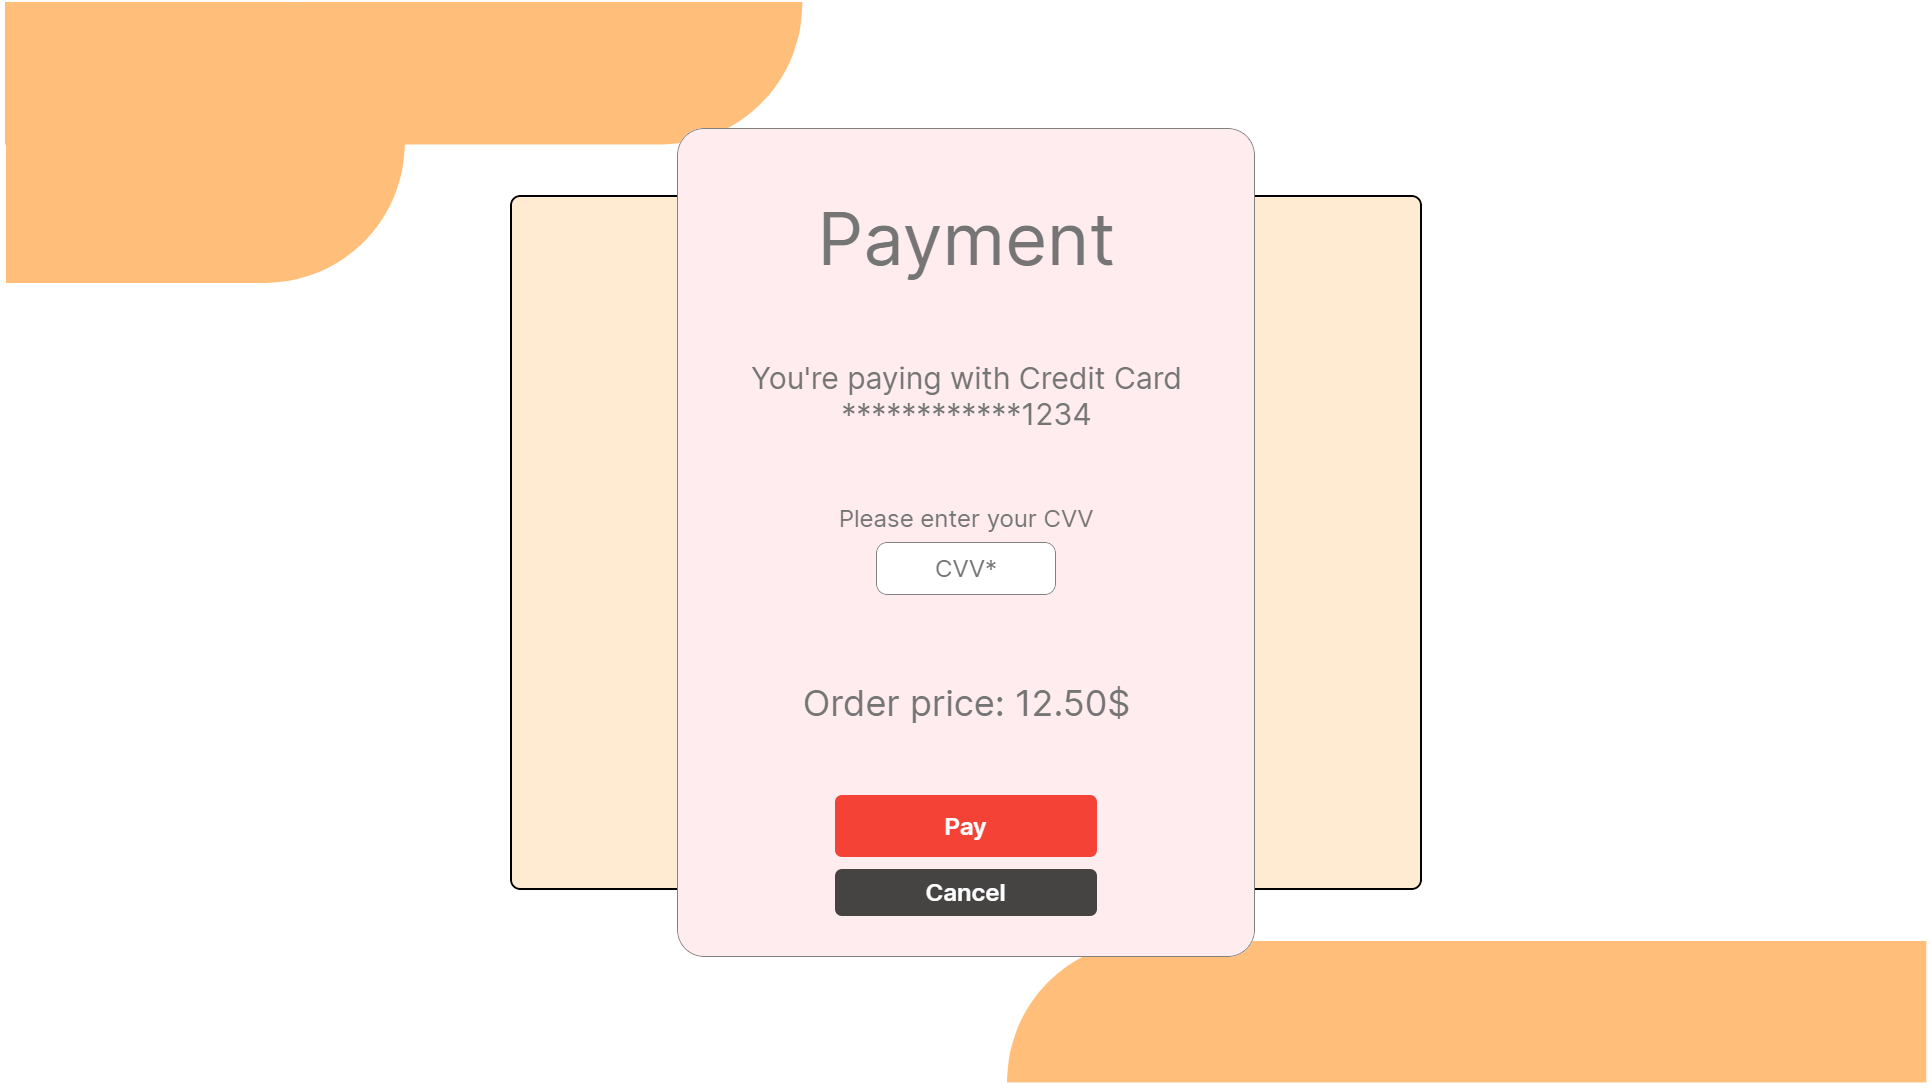
\includegraphics[width=\textwidth]{imgs/mockups/MK_5_PaymentPage.png}
                }
                }
                \caption{Mockup della pagina di pagamento di un ordine - MK\#5}
                \label{fig:mk.5}
            \end{figure}            

\setlength{\fboxsep}{0pt}
            \begin{figure}[H]
                \centering
                \resizebox{1\textwidth}{!}{
                \setlength{\fboxsep}{0pt}
                \tcbox[colframe=grey!20,colback=grey!20,boxsep=0mm,arc=1mm]{
                    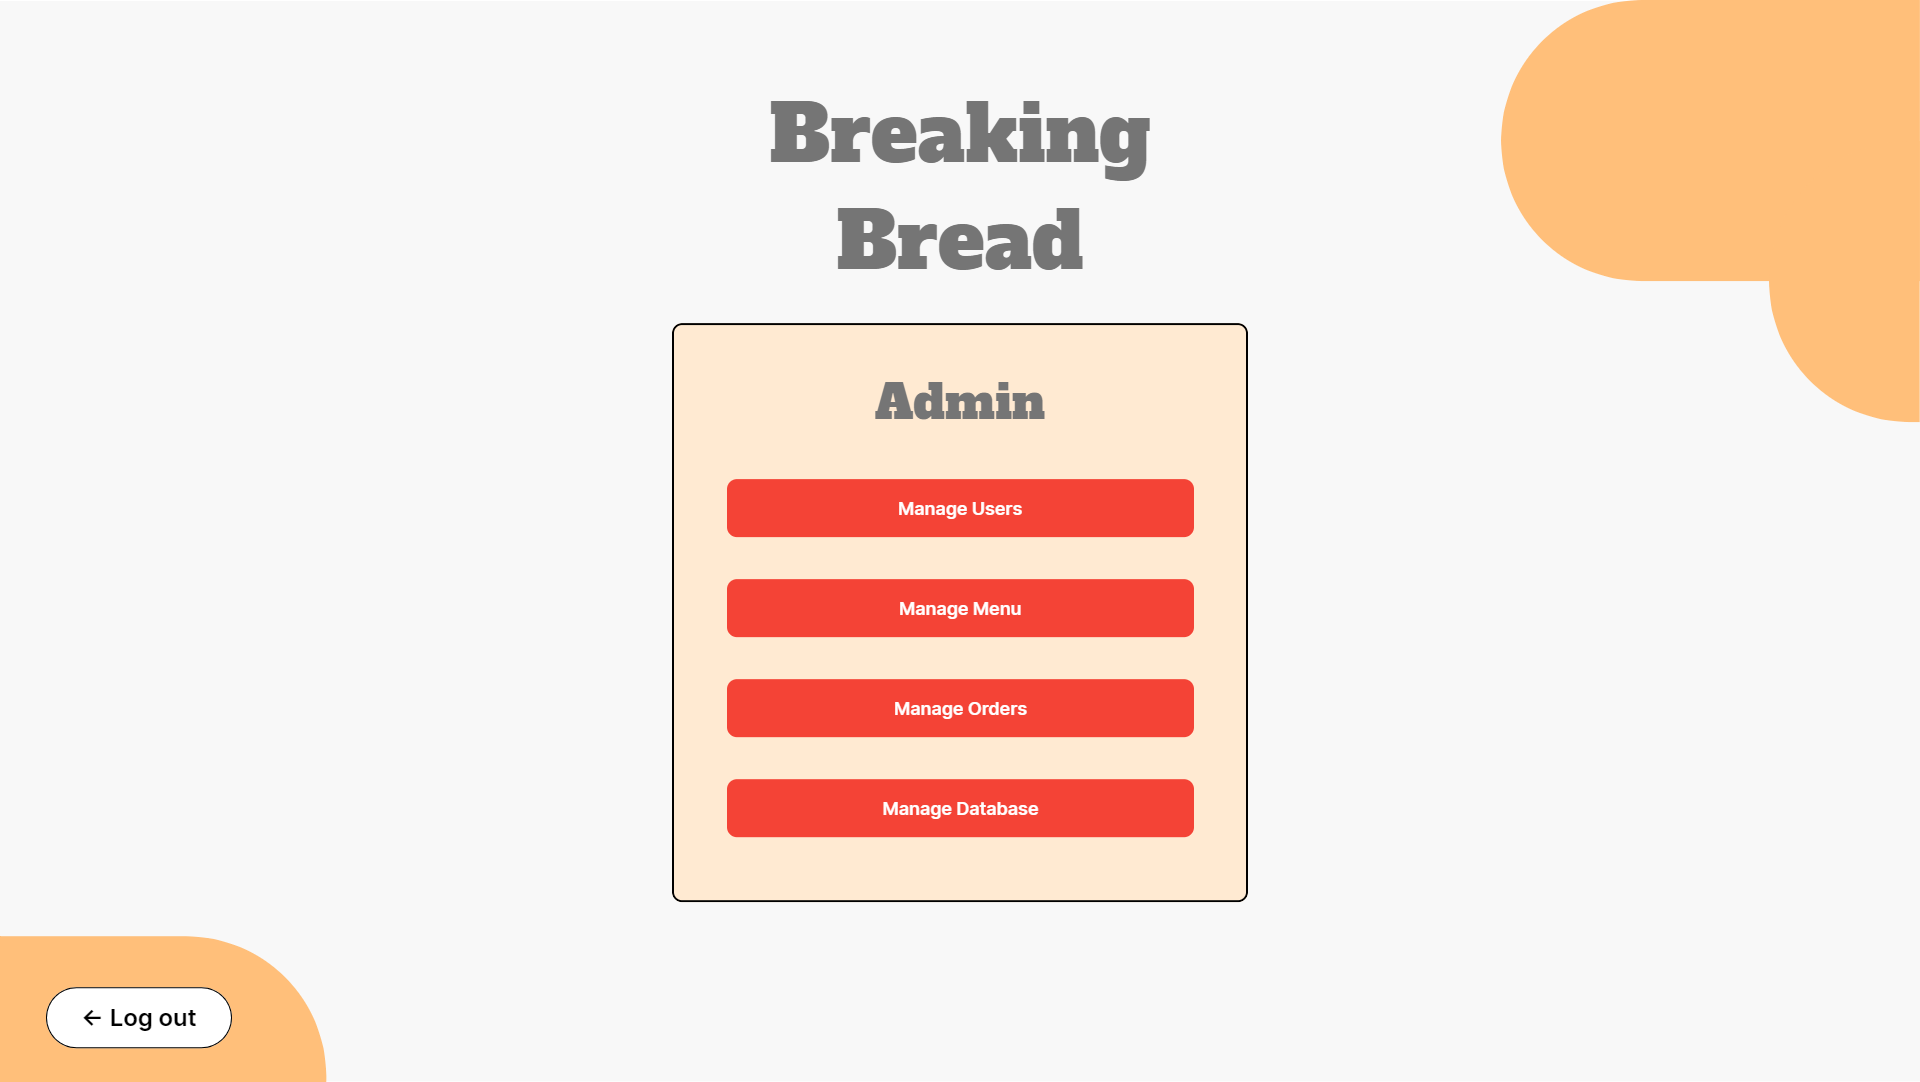
\includegraphics[width=\textwidth]{imgs/mockups/MK_6_AdminPage.png}
                }
                }
                \caption{Mockup della homepage dell'admin - MK\#6}
                \label{fig:mk.6}
            \end{figure}        

\setlength{\fboxsep}{0pt}
            \begin{figure}[H]
                \centering
                \resizebox{1\textwidth}{!}{
                \setlength{\fboxsep}{0pt}
                \tcbox[colframe=grey!20,colback=grey!20,boxsep=0mm,arc=1mm]{
                    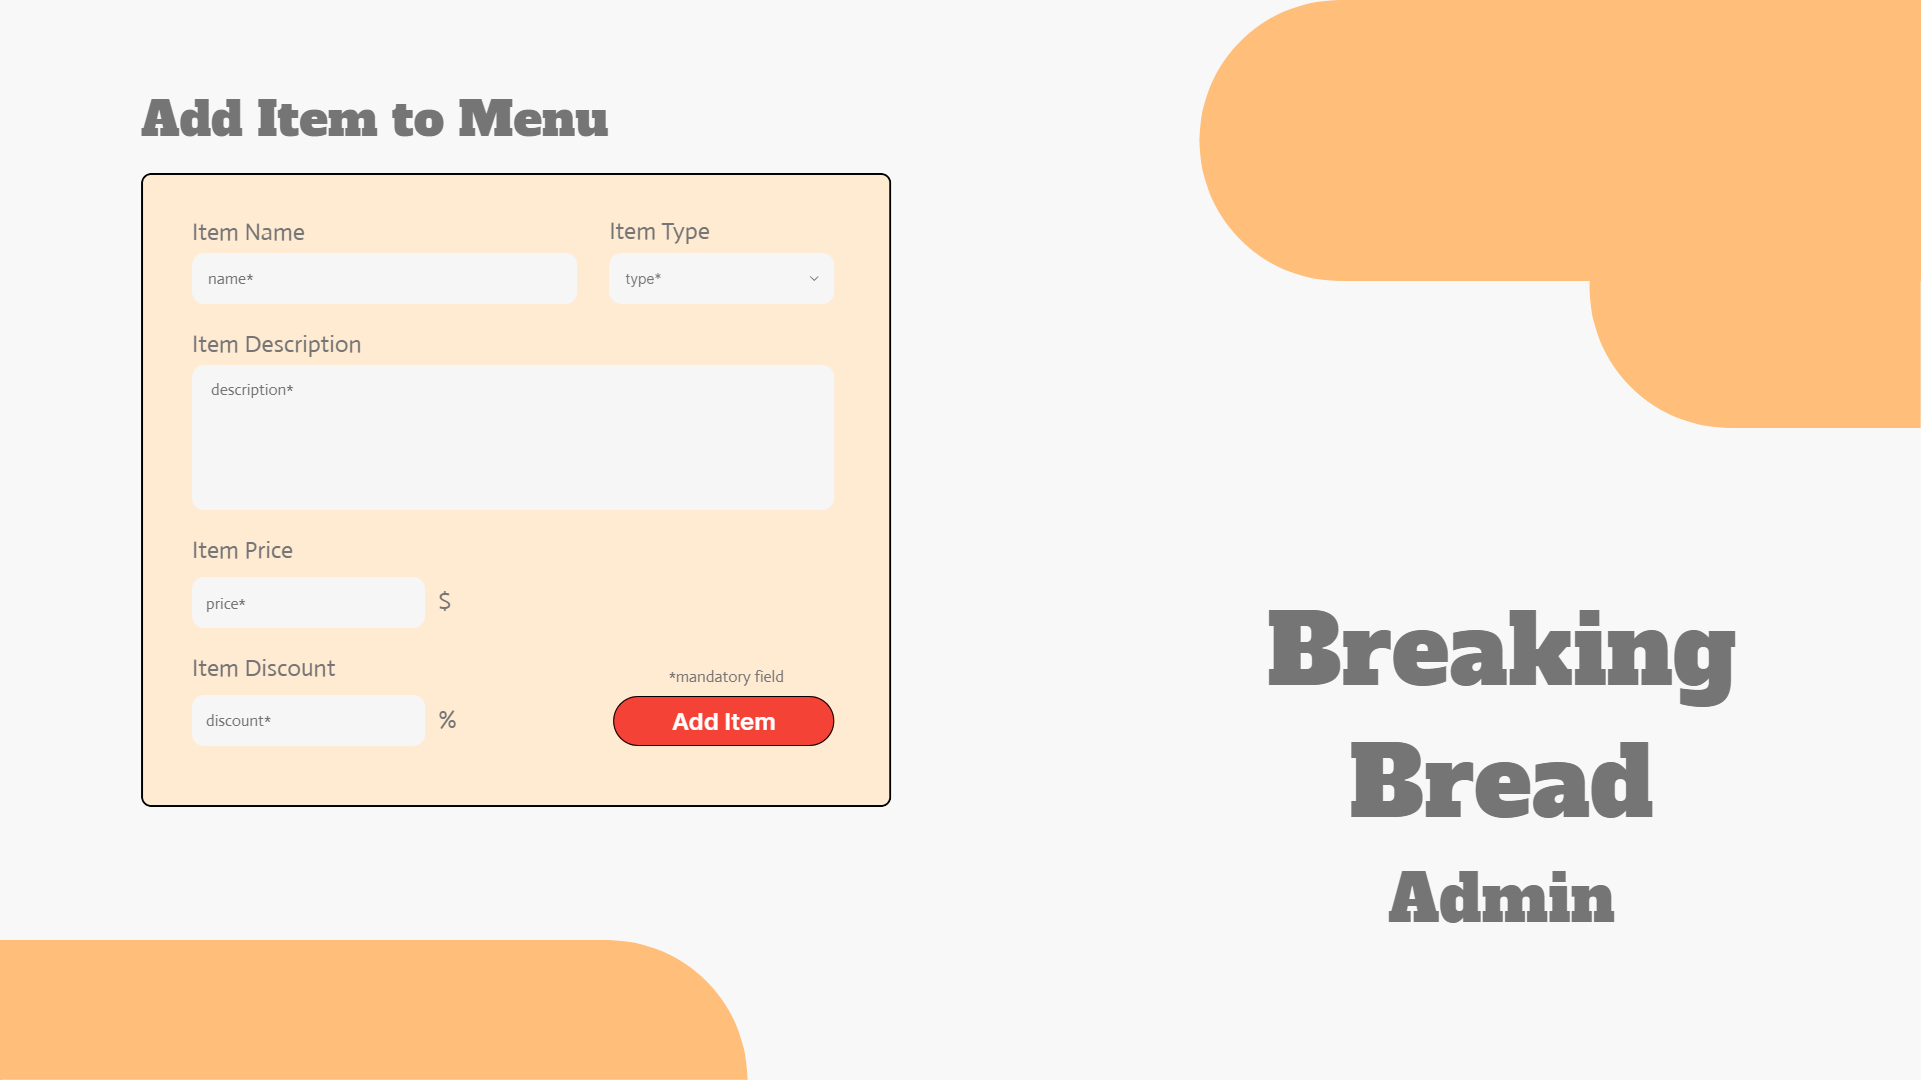
\includegraphics[width=\textwidth]{imgs/mockups/MK_7_NewItemPage.png}
                }
                }
                \caption{Mockup della pagina per l'aggiunta di una pietanza - MK\#7}
                \label{fig:mk.7}
            \end{figure}       

            
\subsection{Class Diagram}
Il progetto è strutturato in tre packages, con lo scopo di separare le respnsabilità e seguire il principio "Separation of Concerns", l'obiettivo è di avere un codice mantenibile e più facilmente testabile.

\subsubsection{Domain Model}
Il livello Domain Model ha la responsabilità di rappresentare le entità principali (figura \ref{domainModel}), definendo per ognuna i propri attributi e i metodi strettamente legati alla classe, come nel caso del PaymentMethod.

\subsubsection{Business Logic}
La Business Logic (figura \ref{business_logic}) gestisce il comportamento principale del sistema, separando le funzioni tra utenti e amministratori. La sua responsabilità è coordinare le operazioni legate a ordini, gestione del profilo, autenticazione, visualizzazione del menu/offerte, e operazioni amministrative come la gestione del database, utenti, ordini e articoli. In sostanza, definisce le regole e i processi chiave che guidano il funzionamento dell'applicazione. I vari Controller presenti nella Buisness Logic sono divisi per Utilizzatore e per Pagina (esempio: UserManageOrderController è un Controller che gestisce la pagina di gestione degli ordini utilizzata da un Utente). 

\clearpage

\subsubsection{ORM}
Il livello ORM (figura \ref{orm}) ha la responsabilità di gestire l’interazione tra l’applicazione e il database. Fornisce metodi per accedere, salvare, modificare ed eliminare dati riguardanti utenti, ordini, articoli, metodi di pagamento e amministratori. Utilizza un singleton chiamato ConnectionManager per garantire una gestione centralizzata e sicura della connessione al database. In sintesi, questo livello traduce gli oggetti del dominio in dati persistenti nel database e viceversa.

%todo mettere domainModel
% ATTENZIONE c'è confusione

   \begin{figure}[h]
        \centering
        \includegraphics[width=1.0\textwidth]{imgs/DomainModelVer2.png}
        \caption{Domain Model}
        \label{domainModel}
    \end{figure}

    \begin{figure}[h]
        \centering
        \includegraphics[width=1.0\textwidth]{imgs/BusinessLogic.png}
        \caption{Business Logic}
        \label{business_logic}
    \end{figure}

    \begin{figure}[h]
       \centering
       \includegraphics[width=1.0\textwidth]{imgs/ORM.png}
       \caption{ORM}
        \label{orm}
    \end{figure}
\clearpage

\subsection{ER Diagram}
La progettazione del database è stata realizzata attraverso uno schema concettuale ER (Entity-Relationship, figura \ref{er}). In questo diagramma sono raffigurate tutte le entità principali del sistema e le relative relazioni. Lo schema rappresenta la struttura logica del database prima della successiva fase di implementazione "fisica" in PostgreSQL, per la quale abbiamo invece usato uno schema relazionale (figura \ref{RelationalModel}).

\vspace{1cm}

\begin{figure}[h]
    \centering
    \includegraphics[width=1\linewidth]{imgs/ER_m.png}
    \caption{ER Diagram}
    \label{er}
\end{figure}

\begin{figure}
    \centering
    \includegraphics[width=1.0\linewidth]{imgs/RelationalModel.png}
    \caption{Relational Model}
    \label{RelationalModel}
\end{figure}

\newpage

\subsection{Directories}
Il progetto è strutturato in varie directories, divise a seconda del loro scopo. \\
Le principali sono:
\begin{itemize}
    \item {\textbf{docs}}: contiene il report e i vari diagrammi del programma
    \item {\textbf{lib}}: contiene le varie librerie necessarie al programma
    \item {\textbf{src/main}}: contiene le classi Java
    \item {\textbf{src/test}}: contiene le classi per lo Unit Testing
\end{itemize}

\begin{figure}[!h]
    \includegraphics[width=0.5\linewidth]{imgs/Directories.png}
    \centering
    \caption{Directories}
    \label{Directories}
\end{figure}

\clearpage

%_______________________________________________________________________________________
\section{Implementazione}

\subsection{Domain Model}
\subsubsection{User}
La classe "User" rappresenta l'entità utente, definito sugli attributi: id (univoco per ogni utete), name, surname, username, age, sex, email, password, paymentMethod (riferimento alla classe omonima), cart (ArrayList contente id degli item).

\subsubsection{Item}
La classe "Item" rappresenta l'entita pietanza, definita sugli attributi: itemld (univoco per ogni pietanza), name, type, description, price e discountPercentage.

\subsubsection{PaymentMethod}
La classe "PaymentMethod" rappresenta il metodo di pagamento, in questo caso una carta di credito. E' definita sugli attributi: ownerName, ownerSurname, cardNumber, cardExpirationDate, cardCVV, withheld. Questa classe implementa i metodi : 

\begin{itemize}
    \item \texttt{pay()} il quale prende fra i parametri un riferimento a "order" da cui ricava la il costro totale dell'ordine e si accerta che vengano inseriti correttamente dall'utente i codici per validare il pagamento.

    \item \texttt{refund()} questo metodo verifica che sull'ordine che riceve fra i parametri si possa effettuare un rimborso, basandosi sull'attrbuto status di "Order".
\end{itemize}

\subsubsection{Order}
La classe "Order" rappresenta un ordine, è definito sugli attributi: orderld(univoco per ogni ordine), status, user, date e items(ArrayList di "Item"). La classe "Order" realizza un design pattern Mapper, il quale ha la responsabilità di mappare un User con molteplici Item presenti nel suo ordine.

\subsubsection{Order Factory}
La classe OrderFactory offre un metodo statico \texttt{createOrder()} per generare oggetti Order già validati, controllando che tutti i parametri richiesti (ID, utente, prodotti, stato e data) siano presenti. Questo approccio standardizza la creazione degli ordini (figura \ref{orderFactory})


\begin{figure}[h]
    \includegraphics[width=1.0\linewidth]{imgs/snippets/Code_OrderFactory.png}
    \caption{OrderFactory}
    \label{orderFactory}
\end{figure}

\newpage
%_______________________________________________________________
\subsection{Business Logic}

\subsubsection{LogInController}
Questa classe si occupa di gestire il "Log in" permettendo l'accesso o la registrazione a utenti comuni, mentre garantisce l'accesso all'admin alla sua area riservata.

\subsubsection{UserManageOrderController}
Il compito di questa classe è permettere agli utenti di gestire i propri ordini, sia quelli passati che quello corrente. La gestione è possibile grazie ai metodi: \texttt{addltem()}, \texttt{removeltem()}, \texttt{viewCurrentOrder()}, \texttt{confirmCurrentOrder()}, \\ \texttt{cancelCurrentOrder()}, \texttt{ViewOrders()}, \texttt{cancelOrder()} i quali agiscono solo su gli oridini correnti tranne per gli ultimi due che agiscono su ordini passati,

\subsubsection{UserViewMenuController}
Questa classe permette di visualizzare il menu, una lista di Item, e il menu delle offerte, una lista di Item selezionati fra quelli che hanno il campo "discountPercentage" diveso da zero.

\subsubsection{UserProfileController}
Questa classe permette all'utente di controllare e gestire la prorpia area personale, aggiornado dati vecchi o gestendo metodi di pagamento, necessari per poter effettuare un ordine.

\subsubsection{AdminDatabaseOptionsController}
La AdminDatabaseOptionsController permette all'utente Admin di gestire le proprie credenziali o di svuotare il database.

\subsubsection{AdminUserControl}
In questa area si permette all'utente admin di gestire tutti gli utenti registrati alla applicazione. Qui l'utente Admin ha la possibilità di avere una lista di tutti gli utenti, grazie al metodo \texttt{viewUsers()}.

\subsubsection{Admin Order Controller}
Come la precedente classe anche questa è pensata per l'utente Admin, qui l'Admin ha infatti la possibilità di gestire gli ordini degli utenti attraverso metodi come \texttt{viewOrders()}, \texttt{updateOrderStatus()} o \texttt{cancelOrder()}.

\subsubsection{AdminItemController}
Questa classe, come il nome suggerisce, permette sempre all'utente Admin di gestire gli Item che gli utenti possono ordinare dal menu.




\newpage


%_______________________________________________________________
\subsection{Object-Relational Mapping}
Il package \texttt{main.java.ORM} contiene le classi che si occupano dell'Object-Relational Mapping, ovvero delle operazioni di scrittura e lettura di dati nel database.

\subsubsection{ConnectionManager}
La classe ConnectionManager, la quale implementa un design pattern "Singleton" in quanto è richiesta una sola istanza di tale, si occupa dell'importante compito di gestire le connessioni con il database tramite il metodo \texttt{getConnection()}. Questa classe contiene, inoltre, tutti i dati necessari per effettuare l'accesso al database, ovvero l'URL, username e password.

\begin{figure}[!h]
    \includegraphics[width=1.0\linewidth]{imgs/snippets/Code_GetConnection.png}
    \caption{Metodo \texttt{getConnection()}}
    \label{code_getConnection}
\end{figure}

\subsubsection{UserDAO}
La classe UserDAO gestisce gli utenti e la connessione della classe User al database. Questa classe implementa vari metodi, tra cui \texttt{addUser()}, \texttt{removeUser()}, \texttt{verifyPassword()}, alcuni metodi per ottenere i dati da uno o più utenti, come \texttt{getUser()} e \texttt{getAllUsers()}, e vari metodi per l'aggiornamento dei dati personali e di accesso dell'utente.

\begin{figure}[!h]
    \includegraphics[width=1.0\linewidth]{imgs/snippets/Code_ClassUserDAO.png}
    \caption{Costruttore e metodo \texttt{addUser()}}
    \label{code_classUserDAO}
\end{figure}

\subsubsection{AdminDAO}
La classe AdminDAO si occupa di effettuare le operazioni di gestione del database a disposizione dell'Admin. In questa classe abbiamo il metodo \texttt{clearDatabase()}, il quale si occupa dell'esecuzione di una stringa SQL che ripristina il database, e il metodo \texttt{generateDummyData()}, il quale serve per generare dei dati fittizi all'interno del database.

\subsubsection{PaymentMethodDAO}
La classe PaymentMethodDAO gestisce l'inserimento e la cancellazione di metodi di pagamento all'interno del database tramite, rispettivamente, i metodi \texttt{addPaymentMethod()} e \texttt{removePaymentMethod()}.

\begin{figure}[!h]
    \includegraphics[width=1.0\linewidth]{imgs/snippets/Code_ClassPaymentMethod.png}
    \caption{Metodi \texttt{addPaymentMethod()} e \texttt{removePaymentMethod()}}
    \label{code_classPaymentMethodDAO}
\end{figure}

\clearpage

\subsubsection{ItemDAO}
La classe UserDAO gestisce gli item (pietanze) e la connessione della classe Item al database. Tra i vari metodi implementati da questa classe ci sono \texttt{addItem()}, \texttt{removeItem()}, \texttt{getItem()} (che ritorna un item dato l'id), \texttt{getAllItems()} (che ritorna tutti gli items) e \texttt{getAllDiscountedItems()} (che ritorna tutti gli item aventi uno sconto). Ci sono, inoltre, vari metodi che permettono la modifica di alcuni attributi di Item, come \texttt{updateDescription()}, \texttt{updatePrice()} e \texttt{updateDiscount()}.

\subsubsection{OrderDAO}
La classe OrderDAO si occupa di gestire sia la tabella Orders che la tabella OrdersItem (relazione 1:N, che collega un ordine a 1 o più Items). I metodi che implementa la classe sono: \texttt{createOrder()}, \texttt{removeOrder()}, \texttt{removeCompletedOrders()} (il quale rimuove tutti gli ordine con status == "Completed"), \texttt{getOrder()}, \texttt{getAllOrders()}, \texttt{getOrdersByUser()} e \texttt{updateStatus()}. Tutti i metodi "getter" richiedono l'utilizzo di un altro DAO, in particolare dell'ItemDAO. Il metodo \texttt{getAllOrdersByStatus()} riceve in ingresso una variabile booleana e restituisce tutti gli ordini completati se la variabile è "true" oppure tutti gli ordini non ancora completati se la variabile è "false".
Un altro metodo che richiede particolarmente attenzione è il metodo \texttt{createOrderItemFromIds()}: dato un orderId e una lista di itemId, questo metodo popola la tabella OrdersItem inserendo per ciascun articolo il numero di volte che compare nella lista come quantità (quantity); in breve, inserisce nel database gli articoli relativi a un ordine.

\begin{figure}[h]
    \includegraphics[width=1.0\linewidth]{imgs/snippets/Code_CreateOrderItemFromIds.png}
    \caption{Metodo \texttt{createOrderItemFromIds()}}
    \label{code_createOrderItemFromIds}
\end{figure}

\begin{figure}[!h]
    \includegraphics[width=1.0\linewidth]{imgs/snippets/Code_GetAllOrdersByStatus.png}
    \caption{Metodo \texttt{getAllOrdersByStatus()}}
    \label{code_GetAllOrdersByStatus}
\end{figure}

\clearpage

\subsection{Database}
Il database è stato progettato in modo da rispettare i requisiti del sistema e contiene le tabelle \texttt{Users}, \texttt{PaymentMethod}, \texttt{Item}, \texttt{Orders} e \texttt{OrdersItem} (figura \ref{er}).
I file relativi al database sono contenuti in \texttt{src/main/sql} e sono:
\begin{itemize}
    \item {\texttt{database.sql}} , il cui compito è quello di cancellare le vecchie tabelle (tramite il comando \texttt{DROP TABLE IF EXISTS}) e ricrearne nuove (vuote)

    \item \texttt{dummydata.sql} , il quale contiene le istruzioni SQL per l'inserimento di dati fittizi nel database, utili effettuare test più mirati e particolari
\end{itemize}

\begin{figure}[h]
    \includegraphics[width=0.9\linewidth]{imgs/snippets/Code_SQLReset.png}
    \centering
    \caption{Cancellazione di tutte le tabelle e creazione della tabella Users e PaymentMethod}
    \label{code_SQLReset}
\end{figure}

\newpage

\subsection{Command Line Interface}
E' stata sviluppata un’interfaccia a riga di comando per il sistema, il cui codice si trova nel file \texttt{Main.java} (percorso: \texttt{src/main/Main.java}). L’utente può interagire con il programma e accedere alle diverse funzionalità navigando tra le varie schermate tramite i comandi numerati suggeriti dal sistema. Il codice presente nel file \texttt{Main.java} reindirizza l'utente nelle varie pagine a seconda dell'input inserito tramite vari switch-case.


\newpage

\section{Testing}
Il progetto è divisio in tre packages e per ciascuno di questi abbiamo implementato delle classi incaricate di svolgere test sul programma. Le classi di test sono: DomainModelTest, BusinessLogicTest e ORMTest.


\subsection{BusinessLogicTest}
Di seguito sono riportati i test della Business Logic, in viola sono riportati i nomi delle classi, mentre in arancione i metodi di test che queste implementano.


\begin{figure}[!h]
    \centering
    \includegraphics[width=0.4\linewidth]{imgs/BusinessLogicTest.png}
    \caption{BusinessLogicTest}
    \label{BusinessLogicTest}
\end{figure}

Tutte le classi di test implementano un un metodo \texttt{setUp()} e uno \texttt{tearDown()}, questo con lo scopo di mettere i metodi effettivi di test nelle condizioni e con le risose adeguate per verificare il codice. In modo particoalare la \texttt{setUp()} si occupa di allocare gli oggetti e aggiungere occorenze nel database da testare, mentre la \texttt{tearDown()} rimuove dal database le occorenze usate nei test (figura \ref{SetUP-TearDown}).\\ Questo lo si fa per lasciare intonzo il database dopo l'esecusione dei test.


\begin{figure}[H]
    \centering
    \includegraphics[width=1.0\linewidth]{imgs/snippets/SetUp-TearDown.png}
    \caption{Esempio Uso SetUP, TearDown}
    \label{SetUP-TearDown}
\end{figure}

Di seguito sono mostrati i test della LoginControllertest, nei quali
si verifica il corretto fuzionamento dei metodi \texttt{login()} e \texttt{register()} della classe LoginController (figura \ref{LoginControllertest}). Nella  figura \ref{AdminUserControllerTest} è invece riportato il test effettuato sulla classe AdminUserController, nella quale si verficano i metodi \texttt{removeUser()} e \texttt{serachUser()}


\begin{figure}[!h]
    \centering
    \includegraphics[width=1.0\linewidth]{imgs/snippets/testLogin.png}
    \caption{LoginControllertest}
    \label{LoginControllertest}
\end{figure}


\begin{figure}[!h]
    \centering
    \includegraphics[width=1.0\linewidth]{imgs/snippets/AdminUserControllerTest.png}
    \caption{AdminUserControllerTest}
    \label{AdminUserControllerTest}
\end{figure}

\newpage


\subsection{DomainModelTest}
La classe DomainModelTest ha il compito di effettuare test relativi alle classi del DomainModel. Sono stati eseguiti i seguenti test (figura \ref{DomainModelTest}), i quali si concentrano particolarmente sulle classi Order e PaymentMethod dato che queste sono le uniche (nel DomainModel) ad avere metodi più complessi oltre a getters e setters.


\begin{figure}[!h]
    \centering
    \includegraphics[width=0.5\linewidth]{imgs/snippets/DomainModelTest.png}
    \caption{DomainModelTest}
    \label{DomainModelTest}
\end{figure}

A seguire sono rirportati alcuni dei test sulla classe "Order". In figura \ref{OrderTest} sono riportati i test: \texttt{testGetTotal()}, \texttt{testGetTotalWithEmptyItems()}, \texttt{testGetTotalWithSingleItem()}.

\begin{figure}[H]
    \centering
    \includegraphics[width=1.0\linewidth]{imgs/snippets/OrderTest.png}
    \caption{OrderTest}
    \label{OrderTest}
\end{figure}

\subsection{ORMTest}
Il package ORMTest si occupa di effettuare i test sulle classi contenute nel package ORM. Sebbene alcuni metodi siano già stati testati in modo indiretto nel package BusinessLogicTest, è stato comunque deciso, per completezza, di creare un package di test dedicato.

\begin{figure}[H]
    \centering
    \includegraphics[width=1.0\linewidth]{imgs/snippets/Code_ItemDAOTest.png}
    \caption{ItemDAOTest}
    \label{ItemDAOTest}
\end{figure}

\begin{figure}[H]
    \centering
    \includegraphics[width=1.0\linewidth]{imgs/snippets/Code_OrderDAOTest.png}
    \caption{OrderDAOTest}
    \label{OrderDAOTest}
\end{figure}


\end{document}
